\section{Robot Arms and Mobile Robots}

\subsection{Types of robots considered}

In this course, we consider two main categories of robots: \textbf{robotic arms}, i.e., stationary manipulators used for tasks such as welding, painting, and assembly, and \textbf{mobile robots}, autonomous ground vehicles used to transport goods or navigate industrial environments.

Both categories may be either \textbf{collaborative}—designed to work safely alongside humans without fencing or physical barriers—or \textbf{non-collaborative}, operating in isolated or restricted areas due to safety concerns.

\begin{figure}[H]
  \centering
  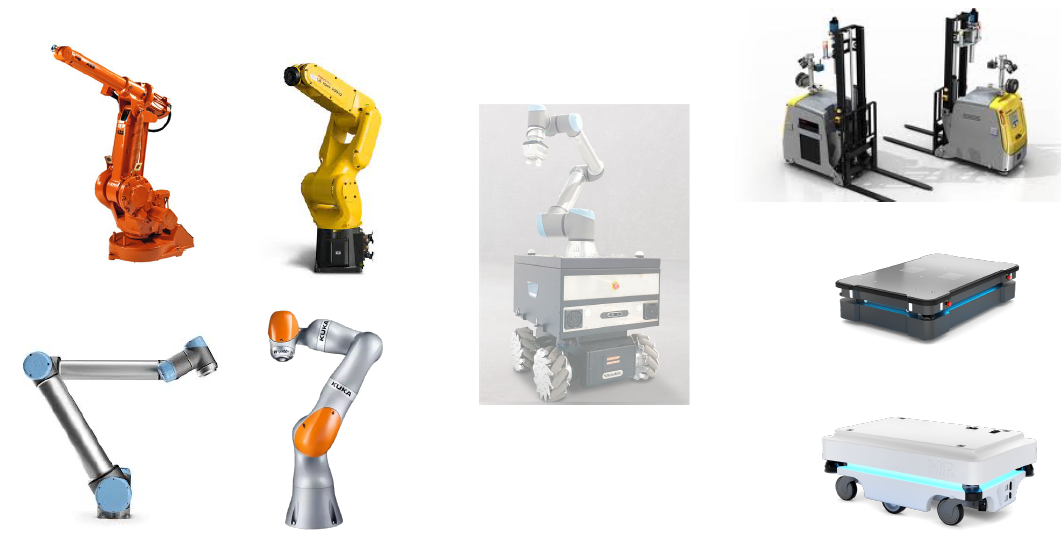
\includegraphics[width=\linewidth]{imgs/robot_types.png}
  \caption{Examples of robotic arms (top left), collaborative arms (bottom left), mobile robots (right), and integrated mobile manipulators (center).}
\end{figure}

\hfill

\subsection{Robotic Arms}

A robotic system is composed of two main components: the \textbf{control system}, an electronic unit that processes commands, plans motion and interfaces with the environment and the user—typically through a \textbf{teach-pendant}—and the \textbf{manipulator}, the mechanical structure, often an articulated arm, that physically interacts with the environment by moving, gripping or assembling objects. These two parts are strongly interconnected and operate together to enable robotic functionality.

\begin{figure}[H]
  \centering
  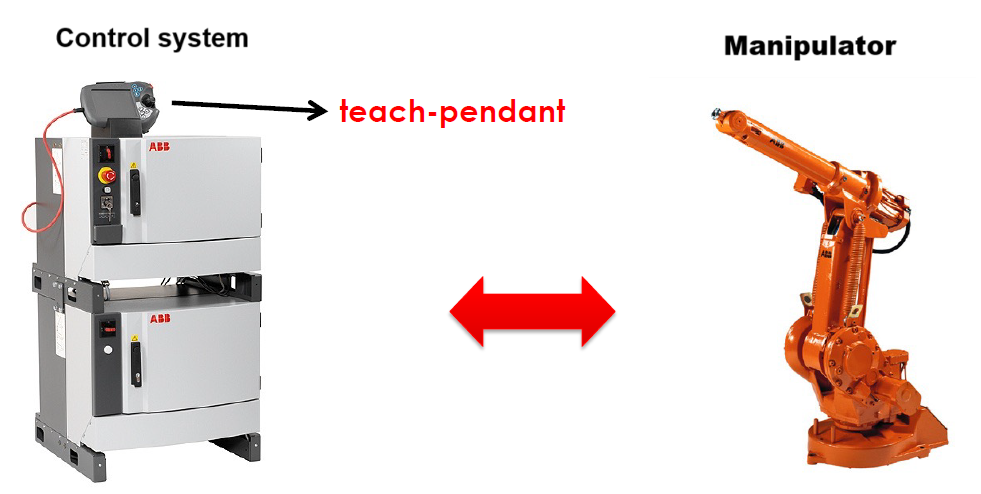
\includegraphics[width=0.7\linewidth]{imgs/robotic_arm_structure.png}
  \caption{Composition of a robot: the control system (left, with teach-pendant) and the mechanical manipulator (right).}
\end{figure}

\hfill

\subsection{The control system}

The control system is considered the \textbf{``brain''} of the robot. Its main role is to determine the motions that the manipulator should perform, combining the assigned task, information received from sensors and internal control algorithms.

It is generally a \textbf{complex architecture}, composed of multiple processors and often connected to various devices for monitoring, control, and data storage. Among its fundamental functions are the human interface, which allows operators to interact with the robot (for instance via a teach pendant), data storage for configurations and programs, motion planning, real-time joint control and continuous sensor monitoring.

\hfill

\subsection{The manipulator}

The manipulator is the part of the robot that directly interacts with the external environment. It is typically composed of a series of rigid bodies called \textbf{links} interconnected by actuated \textbf{joints}. The manipulator is anchored by a \textbf{base}, which can either be fixed to the ground or mounted on a mobile platform.

At the opposite end it usually features an \textbf{end-effector}—the component that performs the actual work, such as grippers, welders or anthropomorphic hands. The end-effector is mounted on the \textbf{wrist}, a joint that provides orientation and fine rotation capabilities to the tool.

\begin{figure}[H]
  \centering
  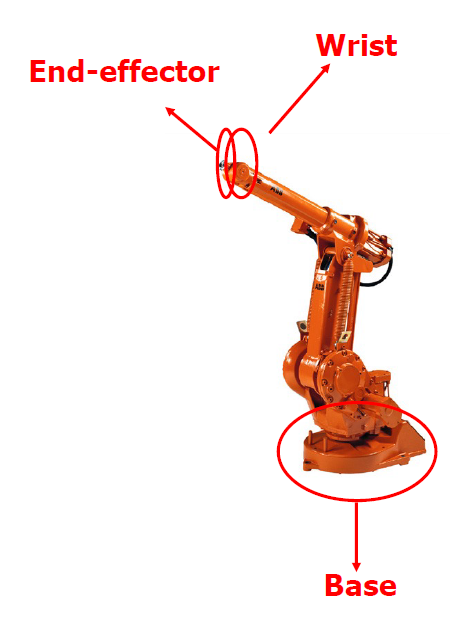
\includegraphics[width=0.35\linewidth]{imgs/manipulator_labeled.png}
  \caption{Main components of a robotic manipulator: base, wrist, and end-effector.}
\end{figure}

\subsection{Common mechanical structures for robotic arms}

Several mechanical structures can be adopted for building a robotic arm. The most common ones are:

\begin{itemize}
  \item \textbf{Cartesian configuration}: composed of three linear axes (X, Y, Z). It is suitable for tasks that require high precision and repeatability in a cuboidal workspace.
  \item \textbf{Cylindrical configuration}: includes one rotary joint at the base and two linear movements. It provides access to a cylindrical workspace.
  \item \textbf{SCARA configuration (Selective Compliance Articulated Robot Arm)}: designed primarily for horizontal movement, combining rotary and linear motions.
  \item \textbf{Anthropomorphic configuration (or articulated arm)}: resembles the human arm, with several rotary joints providing high flexibility and reachability.
\end{itemize}

\begin{figure}[H]
  \centering
  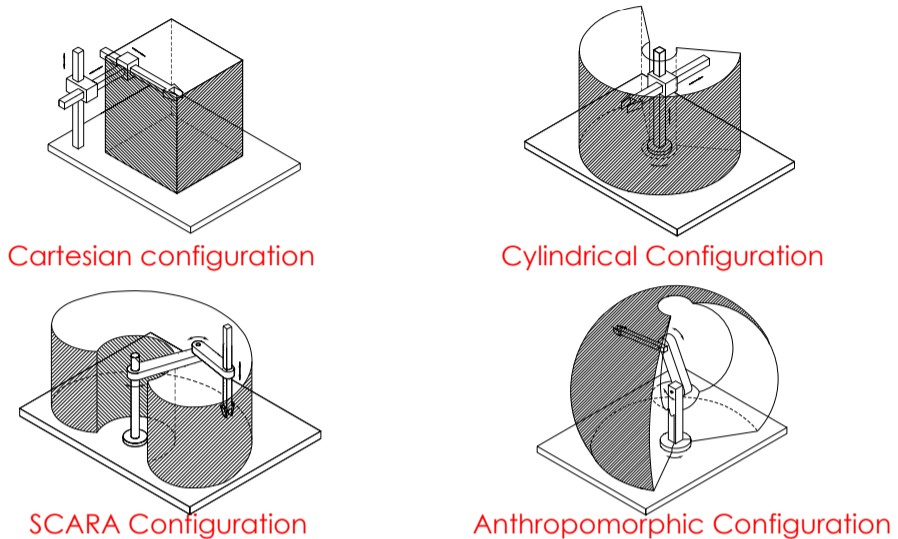
\includegraphics[width=0.8\linewidth]{imgs/mechanical_structures_schematic.png}
  \caption{Schematic representation of different mechanical configurations: Cartesian, Cylindrical, SCARA, and Anthropomorphic.}
\end{figure}

\begin{figure}[H]
  \centering
  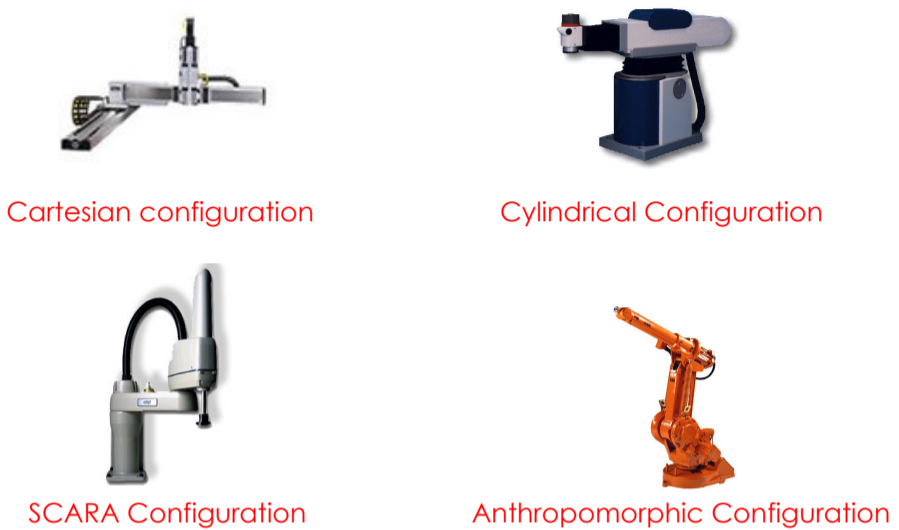
\includegraphics[width=0.8\linewidth]{imgs/mechanical_structures_real.png}
  \caption{Real-world examples of the same mechanical configurations.}
\end{figure}

Among these, the two most common configurations are the Cartesian and the Anthropomorphic ones:

\begin{itemize}
  \item The \textbf{Cartesian structure} is very robust and ideal for transporting heavy loads with high repeatability. However, it tends to be bulky and lacks dexterity.
  \item The \textbf{Anthropomorphic structure} is less robust and has lower payload capacity. Nevertheless, it is compact and offers high dexterity, enabling it to reach distant and complex positions.
\end{itemize}

\hfill

\subsection{Workspace}

The \textbf{workspace} (also called \textbf{task space}) of a robot is the set of all points that its end-effector can reach.

The shape and size of the workspace depend on:
\begin{itemize}
  \item The dimensions of the robot's links;
  \item The type and number of joints;
  \item The mobility limits of each joint.
\end{itemize}

Understanding the workspace is essential for determining the capabilities of a robot in performing tasks within its physical range.

\begin{figure}[H]
  \centering
  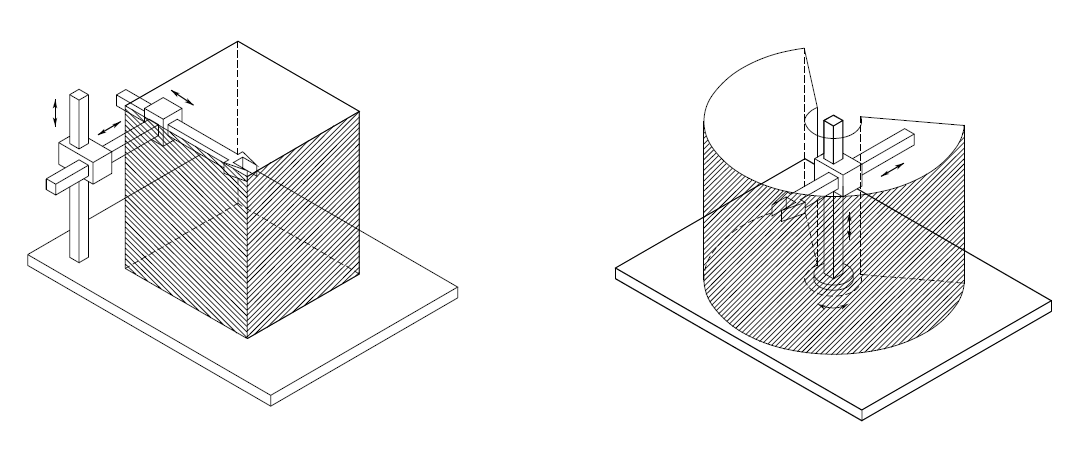
\includegraphics[width=0.85\linewidth]{imgs/workspace.png}
  \caption{Examples of workspace for Cartesian (left) and cylindrical (right) robot configurations.}
\end{figure}

\hfill

\subsection{Joints}

A \textbf{joint} allows a relative motion between two connected links in a robotic arm.

There are two primary types of joints:
\begin{itemize}
  \item \textbf{Prismatic joint} (T): allows linear translation between links;
  \item \textbf{Rotational joint} (R): allows angular rotation between links.
\end{itemize}

More complex joints—such as \textbf{spherical} or \textbf{helicoidal} joints—can be realized through combinations of rotational and/or prismatic joints.  
For instance, a spherical joint can be implemented using three intersecting rotational joints.

Mechanical configurations can also be identified by the sequence of joint types they use. Common notations include:

\begin{itemize}
  \item \textbf{TTT}: Three prismatic joints (Cartesian structure);
  \item \textbf{RT}: One rotational and one prismatic joint (Cylindrical structure);
  \item \textbf{RRT}: Two rotational and one prismatic joint (SCARA structure);
  \item \textbf{RRR}: Three rotational joints (Anthropomorphic structure).
\end{itemize}

\begin{figure}[H]
  \centering
  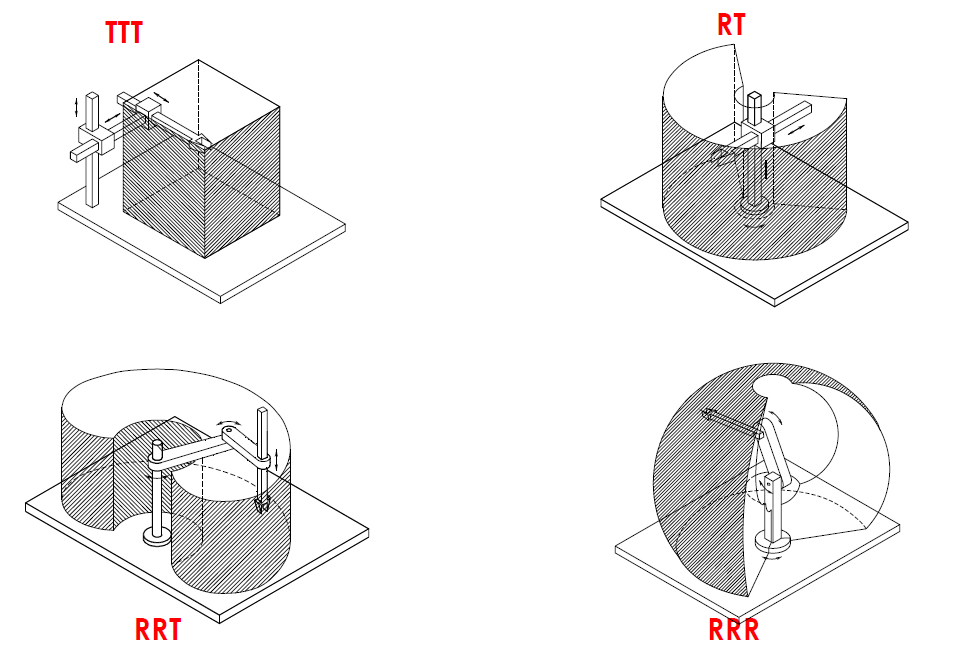
\includegraphics[width=0.8\linewidth]{imgs/joint_configurations.png}
  \caption{Joint configurations for common robot types: TTT, RT, RRT, and RRR.}
\end{figure}

\hfill

\subsection{Degrees of Freedom (DOFs) of a manipulator}

The \textbf{degrees of freedom (DOFs)} of a robotic arm correspond to the number of independent movements the robot can perform, which is typically equal to the number of joints.

\begin{itemize}
  \item For simple manipulators: DOFs = number of joints.
  \item For more complex mechanisms, DOFs can be calculated using the \textit{Gruebler formula}.
\end{itemize}

Intuitively, DOFs describe how the end-effector can move in space. The maximum DOFs required to fully control the position and orientation in 3D space is 6 (3 for translation, 3 for rotation).

Let $n$ be the number of joints and $m$ the dimension of the task space:
\begin{itemize}
  \item If $n = m$: the robot can reach any position and orientation — this is a fully controlled system.
  \item If $n < m$: the robot is \textbf{defective}, unable to cover the full workspace with all orientations.
  \item If $n > m$: the robot is \textbf{redundant}, offering multiple ways to reach the same point.
\end{itemize}

\begin{figure}[H]
  \centering
  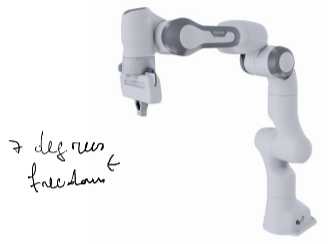
\includegraphics[width=0.4\linewidth]{imgs/franka_panda.png}
  \caption{Franka Emika Panda robot: an example of a redundant manipulator with 7 degrees of freedom.}
\end{figure}

\begin{figure}[H]
  \centering
  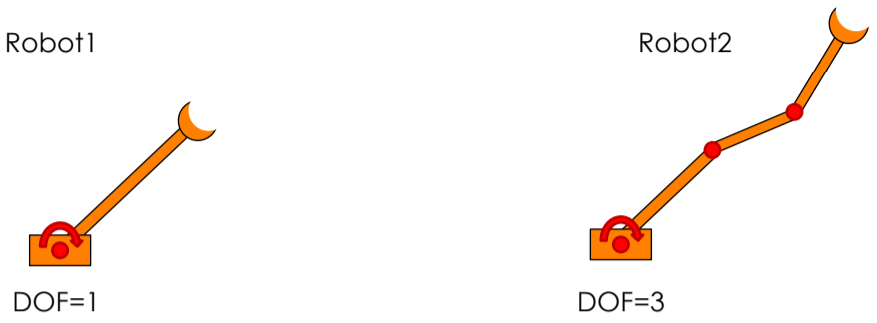
\includegraphics[width=0.8\linewidth]{imgs/dof_examples.png}
  \caption{Simple visual examples: Robot1 with 1 DOF and Robot2 with 3 DOFs.}
\end{figure}

\hfill

\subsection{Joint space and Workspace}

Each joint in a robot is actuated, meaning it is possible to independently control its position. 

To each joint is associated a \textbf{joint variable} $q_i$, which defines the relative position of the $i$-th link with respect to the previous one.

The set of all possible combinations of joint variables defines the \textbf{joint space} of the robot.

In general, if a robot has $n$ joints, its joint space is:
\[
q = 
\begin{pmatrix}
q_1 \\
\vdots \\
q_n
\end{pmatrix}
\in \mathbb{R}^n
\]

\begin{figure}[H]
  \centering
  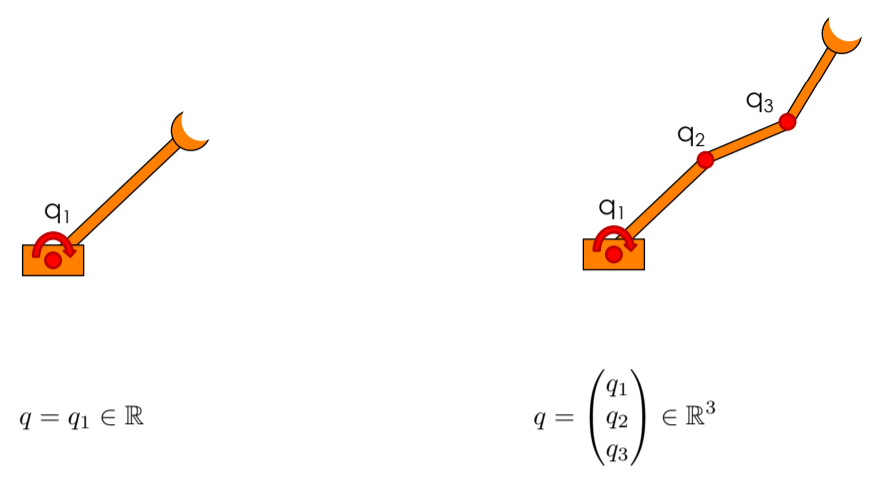
\includegraphics[width=0.9\linewidth]{imgs/joint_space_example.png}
  \caption{Example of joint space: one-joint system with $q_1 \in \mathbb{R}$ (left), and a three-joint system with $q \in \mathbb{R}^3$ (right).}
\end{figure}

\hfill

\subsection{Mobile Robots}

In mobile robots, the control system is integrated directly into the robot. These systems can also receive inputs from external devices, such as a remote control unit.

\subsubsection*{Wheeled Mobile Robots}

Wheels are considered the most appropriate solution for many mobile robot applications. A configuration with three wheels is sufficient to guarantee static stability. The number and type of wheels, as well as their arrangement, depend on the specific application requirements. In this course, the focus will be on Wheeled Mobile Robots (WMR), since they are the most widely used type of industrial mobile robots.

\subsubsection*{Types of wheels}

Wheeled mobile robots can be equipped with different types of wheels, each offering distinct motion capabilities: the \textbf{fixed wheel} allows rolling along its axis but not rotation about the vertical axis; the \textbf{adjustable centered wheel}, similar to a caster but with the pivot axis centered on the wheel, can rotate about the vertical axis; the \textbf{castor wheel} is unpowered and swivels for passive support; finally, the \textbf{omnidirectional wheel} uses rollers mounted around its circumference to permit motion in any planar direction.

\begin{figure}[H]
  \centering
  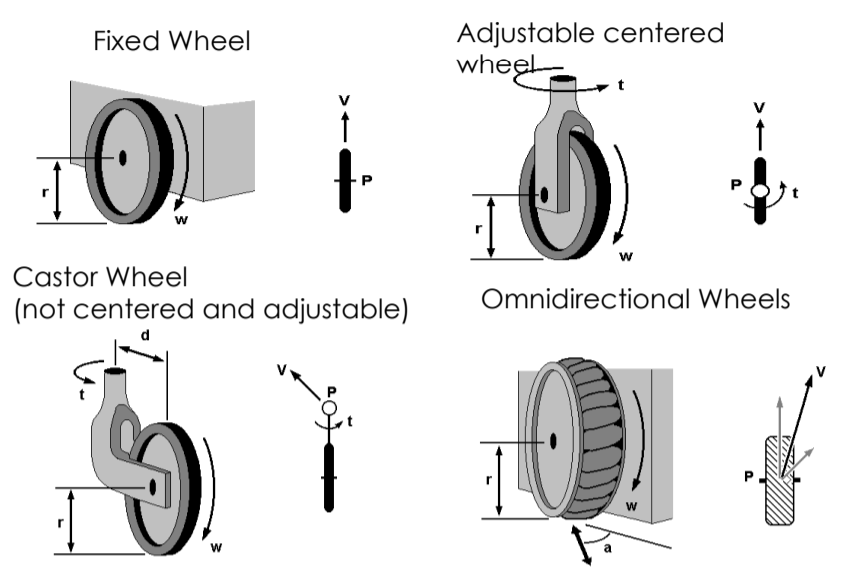
\includegraphics[width=0.9\linewidth]{imgs/types_of_wheels.png}
  \caption{Different types of wheels: fixed, adjustable centered, castor, and omnidirectional.}
\end{figure}

\subsubsection*{Omnidirectional Wheels}

Omnidirectional wheels exploit friction in a controlled manner to generate a transversal component of motion. This allows the robot to move laterally without changing its orientation.

These wheels are equipped with small rollers mounted around the circumference, which rotate independently and enable smooth sideways movement.

\begin{figure}[H]
  \centering
  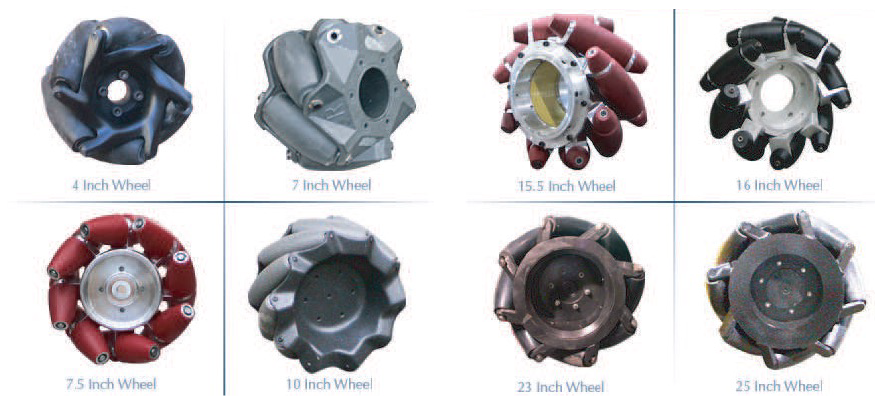
\includegraphics[width=\linewidth]{imgs/omnidirectional_wheels.png}
  \caption{Examples of omnidirectional wheels and their application in mobile robots.}
\end{figure}

\subsubsection*{Most Common Mechanical Structures}

\paragraph{Differential Drive} \hfill

The \textbf{differential drive} is one of the most common configurations for wheeled mobile robots. It consists of two independently actuated coaxial fixed wheels, which are used for both driving and steering.

To ensure static equilibrium, a third passive \textbf{castor wheel}—usually smaller than the actuated ones—is added.

Let $\omega_R$ and $\omega_L$ be the angular velocities of the right and left wheels respectively:
\begin{itemize}
  \item If $\omega_R = \omega_L$, the robot translates straight.
  \item If $\omega_R = -\omega_L$, the robot rotates in place.
  \item Intermediate values result in a general motion called \textbf{rototranslation}.
\end{itemize}

\begin{figure}[H]
  \centering
  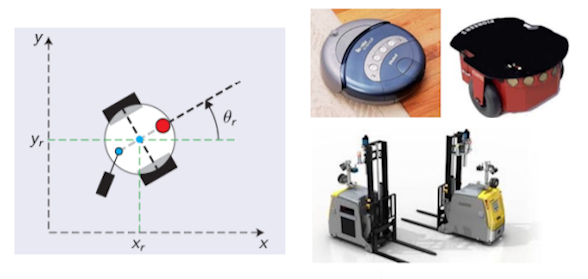
\includegraphics[width=0.8\linewidth]{imgs/differential_drive.png}
  \caption{Differential drive: top-view diagram and examples of real robots using this configuration.}
\end{figure}

Another common set of mechanical structures for wheeled mobile robots includes the \textbf{tricycle} and \textbf{car-like} configurations.

\paragraph{Tricycle} \hfill

This structure has two fixed back wheels and one steering front wheel. It can be either front- or rear-wheel driven.

\begin{itemize}
  \item \textbf{Pro:} High payload capacity.
  \item \textbf{Con:} Limited agility in maneuvering.
\end{itemize}

\paragraph{Car-like} \hfill

It has two fixed and aligned rear wheels and two steering, aligned front wheels. It can also be either front- or rear-wheel driven.

\begin{itemize}
  \item \textbf{Pro:} High payload capacity.
  \item \textbf{Con:} Limited agility in maneuvering.
\end{itemize}

\begin{figure}[H]
  \centering
  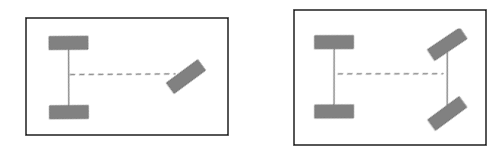
\includegraphics[width=0.85\linewidth]{imgs/tricycle_car_like.png}
  \caption{Mechanical structures: tricycle configuration (left) and car-like configuration (right).}
\end{figure}

\hfill

\subsection{Configuration Space}

The \textbf{configuration} of a robot is a complete specification of the position of every point of the robot.

The set of all possible configurations forms an $n$-dimensional space called the \textbf{configuration space} or \textbf{C-space}.

Each configuration corresponds to a single point in the configuration space.

Since the robot is composed of rigid bodies of known shape, only a limited number of \textbf{configuration parameters} are required to fully define the configuration.

\begin{figure}[H]
  \centering
  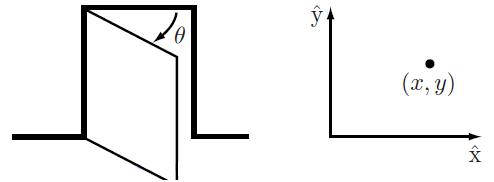
\includegraphics[width=0.55\linewidth]{imgs/configuration_space.png}
  \caption{Examples of configuration representation: position $(x, y)$ and orientation $\theta$.}
\end{figure}

For \textbf{robotic arms}, the configuration parameters are the joint variables $q_i$. In this case, the configuration space coincides with the \textbf{joint space}, represented as:
\[
q = 
\begin{pmatrix}
q_1 \\
\vdots \\
q_n
\end{pmatrix}
\in \mathbb{R}^n
\]

For \textbf{mobile robots}, the configuration parameters must describe the position and orientation of all relevant moving parts. For example:
\begin{itemize}
  \item A differential-drive robot may be described by $q = [x_r, y_r, \theta_r]^T \in \mathbb{R}^3$;
  \item A more complex mobile robot may require $q = [x_r, y_r, \theta_r, \phi_r]^T \in \mathbb{R}^4$.
\end{itemize}

In both cases, the configuration space (\textbf{C-space}) is the set of all possible configurations that the robot can assume.

\begin{figure}[H]
  \centering
  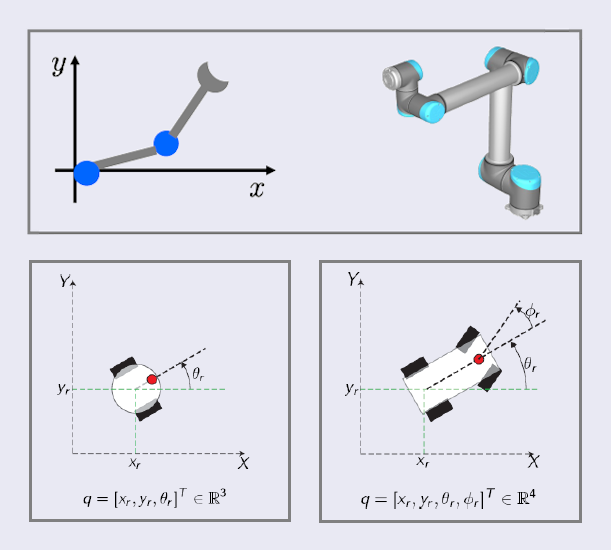
\includegraphics[width=0.9\linewidth]{imgs/configuration_space_examples.png}
  \caption{Configuration space for a robotic arm (top) and mobile robots (bottom left: $\mathbb{R}^3$, bottom right: $\mathbb{R}^4$).}
\end{figure}

\hfill

\subsection{Take-home Message}

Robotic arms and wheeled mobile robots are the most widely used robotic systems in industrial applications.

The most common mechanical configurations for robotic arms are the \textbf{cartesian} and the \textbf{anthropomorphic} ones.

For wheeled mobile robots, the most frequent configurations include the \textbf{differential drive}, the \textbf{tricycle}, and the \textbf{car-like} setups.

Finally, the \textbf{configuration parameters} of a robot define the position of all its parts. For robotic arms, the configuration space (\textbf{C-space}) corresponds to the joint space.

\newpage
